\section{Part VI --- Verification: what was tested and what the tests showed}

\begin{keybox}[The standard]
A modification of a sampler is only worth presenting if (a) the object class is exactly the intended one, (b) the reward is exactly the intended likelihood, (c) the backward policy is exactly a distribution over parents, and (d) the whole thing reduces to the original when the new feature is switched off. Each of the four has an executable test.
\end{keybox}

\subsection{(a) The class: exhaustive enumeration of the MDP}
\file{tests/test\_network\_env.py::test\_class\_counts\_and\_no\_dead\_ends} runs a depth-first search over \emph{all} states reachable from $s_0$ (continuous values ignored; states memoised by a canonical string), collects the terminal networks by canonical string, and checks that every non-terminal state has at least one legal action.
\begin{center}\small
\begin{tabular}{ccrrr}\toprule
$N$ & $R_{\max}$ & reachable terminal networks & expected (Bouvel et al.\ 2020) & distinct states visited \\ \midrule
3 & 2 & 36 & 36 & 205 \\
4 & 1 & 243 & 243 & 1\,001 \\
4 & 2 & 603 & 603 & 4\,829 \\
5 & 1 & 2\,910 & 2\,910 & 12\,821 \\
5 & 2 & 11\,460 & 11\,460 & 109\,131 \\
\bottomrule
\end{tabular}
\end{center}
Dead ends: 0 in every case. The expected numbers are $\sum_{k\le R_{\max}}r(N,k)$ with $r(4,\cdot)=15,228,360$ and $r(5,\cdot)=105,2805,8550$; they were obtained from the published generating function and, independently, from a direct enumeration by insertion (\file{enum\_level1.py}, shipped with the validation material). Three different constructions agreeing on five numbers is as close to a proof-by-computer as this question allows.

\subsection{(b) The likelihood: two vectors versus $2^R$ displayed trees}
\file{src/utils/network\_likelihood.py} is a deliberately slow, independent implementation of eq.~\eqref{eq:netlik}: it enumerates the $2^R$ displayed trees, suppresses degree-2 nodes summing lengths, runs a plain \code{numpy} Felsenstein pass on each, mixes per site, and adds the same edge priors and the reticulation prior. \code{test\_likelihood\_matches\_explicit} draws random networks (random legal actions, random lengths and $\theta$) with $(N,R_{\max})\in\{(4,1),(5,2),(6,3),(7,2)\}$ and compares. Largest absolute difference over 48 networks: $1.5\times10^{-11}$ on log-scores of order $10^3$ --- floating-point agreement.

\subsection{(c) The backward policy}
\code{test\_backward\_sampling\_roundtrip}: for random terminal networks ($N=5,6,8$; $R\le3$), \code{sample\_backward\_from\_network} produces an action list of length $N-1+2R$; replaying it forward reproduces the same canonical network, the same log-score (to $10^{-6}$) and the same sequence of parent counts $|\mathrm{Pa}(s_t)|$ as \code{NetworkState.num\_parents()} computed on the forward states. This is the consistency that trajectory balance relies on.

\subsection{(d) Reduction to PhyloGFN}
With \code{R\_MAX: 0} the environment can only merge; the reward is PhyloGFN's; the policy has the same encoder and pair head (the single head is masked out). \file{tools/compare\_tree\_mode.py} trains the original implementation and the network implementation on the same 6-taxon, 300-site alignment with the same tiny budget (8 epochs $\times$ 40 steps $\times$ 48 trajectories, CPU) and estimates the evidence five times each:
\begin{center}\small
\begin{tabular}{lcc}\toprule
 & MLL (mean $\pm$ s.d.\ of 5 estimates) & wall-clock \\ \midrule
PhyloGFN (original code, \code{ONE\_STEP\_BINARY\_TREE}) & $-1838.92\pm0.38$ & 38 s \\
PhyloGFN-Net with $R_{\max}=0$ & $-1840.97\pm0.29$ & 91 s \\
\bottomrule
\end{tabular}
\end{center}
Both numbers are lower bounds of the same $\log P(\bY)$ (rooted and unrooted uniform priors give the same evidence under a reversible model); the two-unit gap at this budget is training noise (the network code trains fewer effective updates per second, Part~VIII.1). The check that matters is qualitative: the new code path is a functioning PhyloGFN when reticulations are disabled.

\subsection{(e) Learning on simulated data, and the negative control}
\file{tools/simulate\_network\_data.py} generated two 6-taxon, 300-site alignments with the same seed: one on a level-1 network with one reticulation ($\theta=0.5$), one on a tree. Four CPU runs of \file{train\_net.py} ($R_{\max}=2$, batch 48, temperature $8\to1$, $\varepsilon$ $0.5\to0.01$, 12--20 epochs of 40 steps, 10--20 minutes each) are summarised in Fig.~\ref{fig:runs}.

\begin{figure}[h]\centering
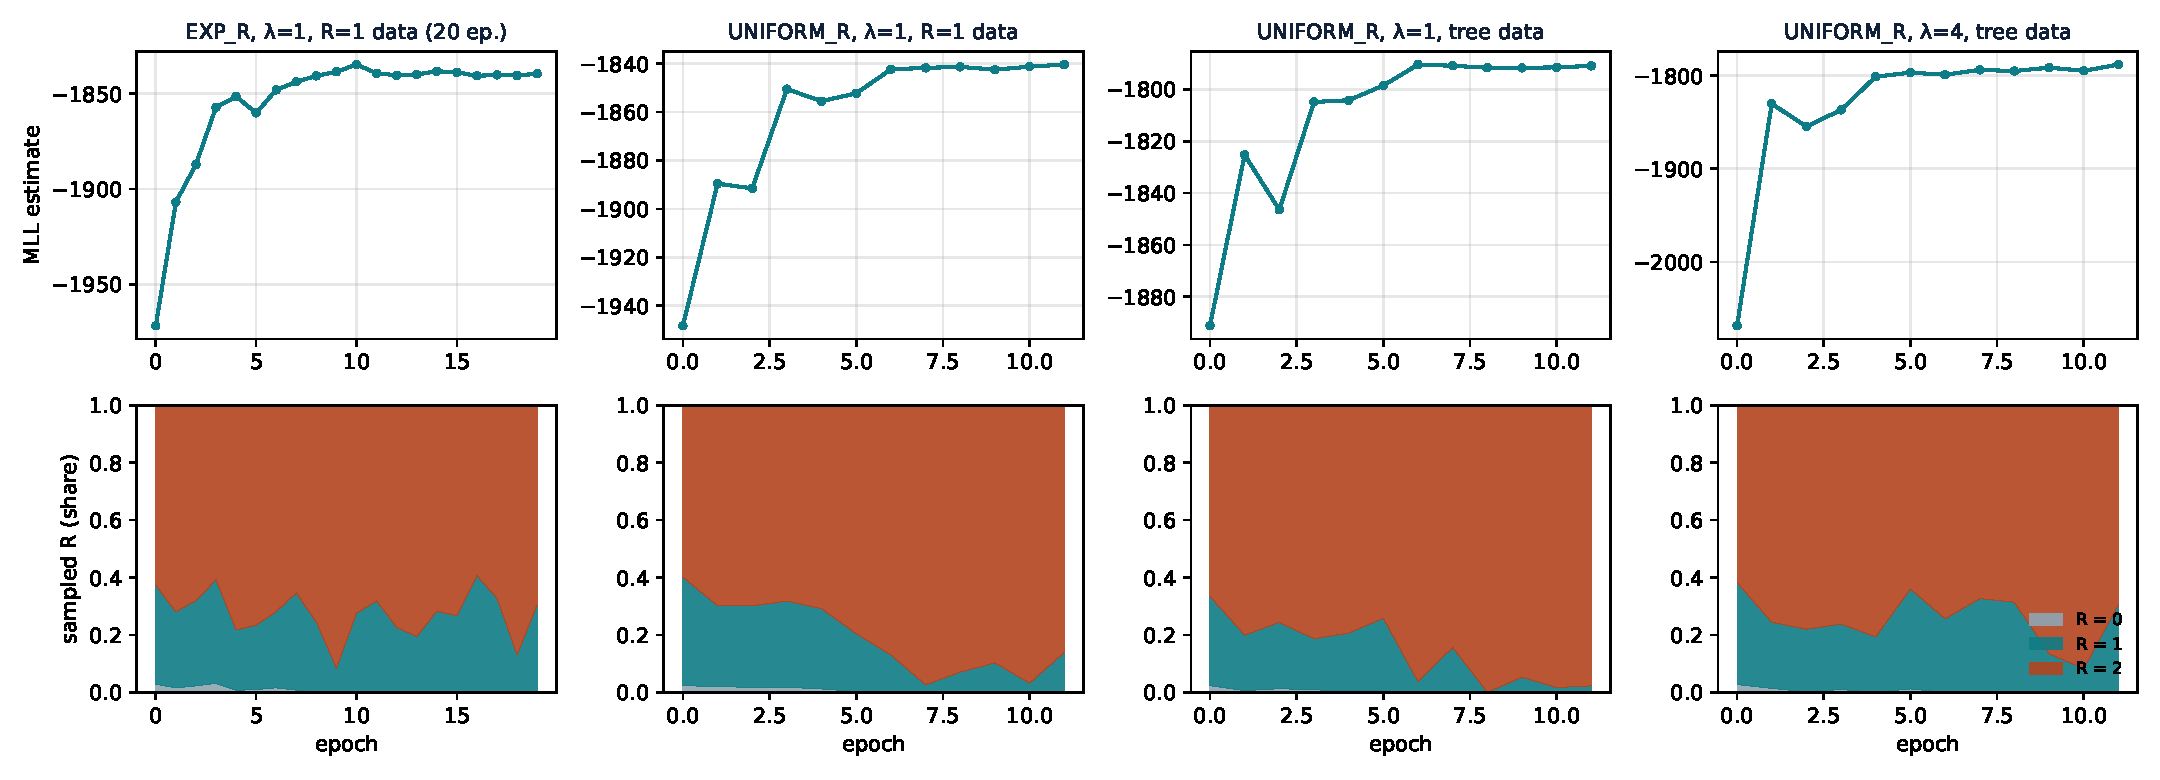
\includegraphics[width=\textwidth]{fig_runs.pdf}
\caption{Top: importance-weighted MLL estimate per epoch. Bottom: share of sampled networks with $R=0,1,2$ reticulations (1\,024 samples per epoch). Left to right: \code{EXP\_R} prior, $\lambda_R=1$, data with one reticulation; \code{UNIFORM\_R}, $\lambda_R=1$, same data; \code{UNIFORM\_R}, $\lambda_R=1$, tree-only data; \code{UNIFORM\_R}, $\lambda_R=4$, tree-only data.}\label{fig:runs}
\end{figure}

\begin{center}\small
\begin{tabular}{llccc}\toprule
data & prior & final MLL & sampled $R$ ($0/1/2$, last epoch) & Pearson $r$ \\ \midrule
$R=1$ & \code{EXP\_R}, $\lambda_R=1$ (20 ep.) & $-1840.6\pm0.6$ & 2 / 310 / 712 & 0.67 \\
$R=1$ & \code{UNIFORM\_R}, $\lambda_R=1$ & $-1842.2\pm0.4$ & 0 / 143 / 881 & 0.55 \\
tree & \code{UNIFORM\_R}, $\lambda_R=1$ & $-1789.8\pm1.5$ & 0 / 24 / 1000 & 0.51 \\
tree & \code{UNIFORM\_R}, $\lambda_R=4$ & $-1792.4\pm0.4$ & 1 / 313 / 710 & 0.65 \\
\bottomrule
\end{tabular}
\end{center}

\paragraph{What works.} The machinery trains: the bound rises by 100--180 log-units during the temperature anneal and then stabilises; the replay buffer fills with high-scoring networks; the two priors and $R_{\max}$ behave as configured; the reduction to PhyloGFN holds.

\paragraph{What does not work yet --- and why it is the right thing to have found.} The negative control (T8 of the validation plan: tree-only data must give posterior mode $R=0$) \emph{fails at this budget}: on tree-simulated data the sampler still returns $R=2$ for 70--98\,\% of its samples, with either prior and even with $\lambda_R=4$. The replay buffers contain no tree at all. The diagnosis is quantitative:
\begin{itemize}[nosep]
\item the true tree with re-optimised branch lengths scores $\log P(\bY\mid G,\bb)+\log P(\bb)=-1757.7$ on the tree data; the best $R=2$ network in the $\lambda_R=4$ buffer scores $-1746.3$ before the topology prior: \emph{12 nats higher};
\item six extra edges ($3R$) with lengths near zero each contribute up to $\log\lambda=\log10=2.3$ nats of prior \emph{density}: the reward is a density over $(G,\bb,\btheta)$ and adding dimensions adds density peaks. The posterior over $R$ is the \emph{integral} of that density over the extra dimensions (an Occam factor that removes the effect), and a converged GFlowNet reproduces the integral. A sampler trained for minutes, with a temperature schedule that first flattens the reward (where the far larger $R=2$ class dominates by volume) and a buffer that stores density peaks, inherits the preference for $R=2$. Pearson $r\approx0.5$--$0.7$ confirms that the fit is still coarse (PhyloGFN reaches $0.99$ after 500 epochs of 1\,000 steps).
\end{itemize}
This is exactly the situation the proposal's validation plan is designed to detect: the exact posterior at $N\le5$ (11\,460 topologies, O3) separates sampler error from prior behaviour; the negative control T8 must pass before any network claim. The prototype delivers the instrument; the remedies are on the roadmap (Part~VIII): longer training with the paper's schedule, the hyper-prior on $\lambda_R$ (or \code{UNIFORM\_R} with $\lambda_R$ set from the exact small-$N$ posterior), and a prior on reticulation edges that does not reward vanishing lengths.
\clearpage
